\chapter{基于邻边卷积网络的复合物筛选模型}
\label{chapter:EdgeConv}
\section{引言}
\label{section:EdgeConv:Put}

已有方法已经充分表明,在PPI网络中进行蛋白质复合物预测不仅仅是一个图论中的聚簇发现问题,更是一个信息融合问题。无论是加权网络方法、核心附属结构预测方法,都致力于最大程度的利用生物学信息进行辅助预测。基于该前提,本文提出了基于生物特征的复合物预测模型。
\section{邻边卷积网络介绍}
\label{section:EdgeConv:intro}



\section{基于邻边卷积网络的复合物筛选模型}
\label{section:EdgeConv:detail}

本文处理了大量的生物学数据,包括蛋白质功能注释数据、结构域相互作用数据、亚细胞定位数据等,应用相关的生物邻域的处理方法将生物学数据转换为可应用的特征数据,最终得到了12维度的特征数据。所有的特征都描述蛋白质相互作用,因此在图结构中,这些特征编码为图结构邻边的特征。

如\ref{section:NodeConv:intro}介绍,已有的图卷积方法为基于结点的卷积算法。在子图结构中,生物信息只能被映射为邻边信息,为了将邻边信息转换为结点信息,本文提出了从邻边到结点的信息汇聚过程。

在通常的图卷积过程中,结点A的特征为周围所有结点的特征和自生特征决定,可以采取平均值的计算方法,如公式\ref{equ:NormalGCNNodeFlow}所示。
\begin{equation}
    \label{equ:NormalGCNNodeFlow}
    f_a=\delta (\frac{\sum_{i = 1}^{n}f_i+f_a}{n+1})
\end{equation}
其中$f_a$代表A结点的特征,$f_i$代表A结点所有邻居的特征,$\delta$为信息汇聚之后的特征更新函数。
在汇聚结点周围邻边的特征计算方法中,结点特征由其邻边共同决定。其具体计算过程如公式\ref{equ:EdgetoNodeFeat}所示。
\begin{equation}
    \label{equ:EdgetoNodeFeat}
    f_a=\delta (\frac{\sum_{i = 1}^{n}f_{ia}}{n})
\end{equation}
其中$f_{ia}$表示所有连接到A的邻边特征。其具体的汇聚过程如图\ref{fig:edge-feat-flow}所示,A结点汇聚周围所有邻边特征,包括$F_{BA}$、$F_{CA}$、$F_{DA}$以及$F_{EA}$。

\begin{figure}[htbp]
    \centering
    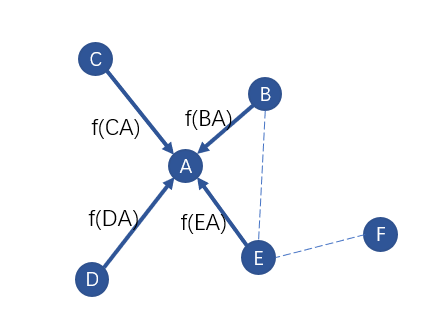
\includegraphics[width=7cm]{edge-feat-flow}
    \caption{边特征初始化结点特征示意图}
    \label{fig:edge-feat-flow}
\end{figure}

蛋白质生物数据是基于邻边的数据,因此在对复合物子图做图卷积的时候,基于生物特征的模型采用了基于edge的GCN模型\cite{wang_dynamic_2019},其具体的邻边更新方式如式\ref{equ:EdgeConv}所示。
\begin{equation}
    \label{equ:EdgeConv}
    h_i^{(l+1)} = \max_{j \in \mathcal{N}(i)} \mathrm{ReLU}(
    \Theta \cdot (h_j^{(l)} - h_i^{(l)}) + \Phi \cdot h_i^{(l)})
\end{equation}
其中$h_i^{(l+1)}$表示第$l+1$层更新之后的结点数据,$h_j^{(l)} - h_i^{(l)}$表示从邻居结点到$i$结点的数据流,$h_i^{(l)}$为结点保留信息,$\Theta$和$\Phi$分别对应更新函数。

\section{算法具体实现与流程}
\label{section:EdgeConv:flow}

首先将生物特征GO注释、拓扑域相似性、亚细胞定位特征整合到一起,嵌入到PPI网络的邻边作为邻边特征。再使用复合物子图抽取方法从网络中获取训练数据集,包括正样本、负样本和中间样本。
然后使用特征汇聚方法将邻边特征汇聚到结点特征中,再使用基于edge更新的图卷积方法进行特征融合。
本文在图分类任务中加上了两层基于邻边的图卷积网络对生物特征和子图拓扑结构进行融合。图读出阶段使用了基于结点的平均池化和最大值池化方法。最终的分类阶段使用了两层感知器模型。
基于生物特征的复合物分类模型总体结构如图\ref{fig:edge-classification-flow}所示。
\begin{figure}[htbp]
    \centering
    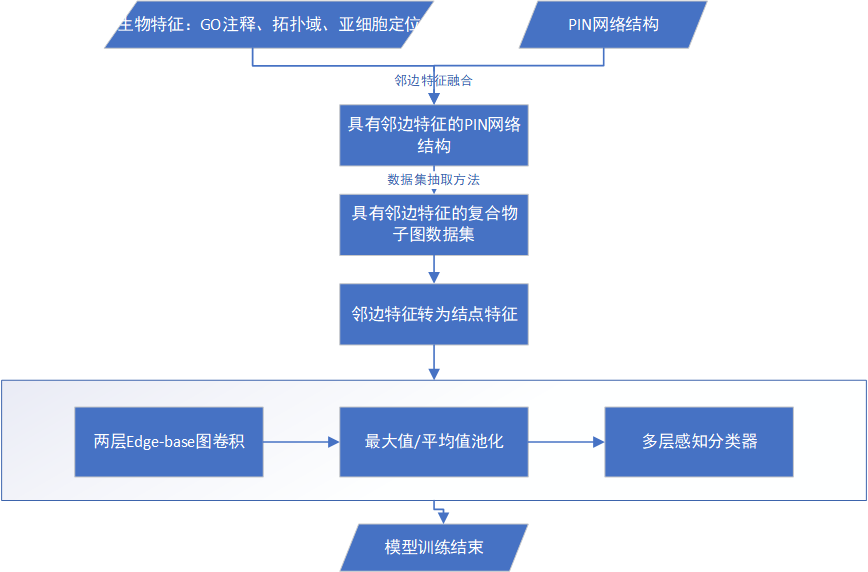
\includegraphics[width=12cm]{edge-classification-flow}
    \caption{基于生物特征的分类模型总体流程}
    \label{fig:edge-classification-flow}
\end{figure}
最终将子图的蛋白质结点特征做平均池化,作为蛋白质复合物特征的输出,以多层感知器预测复合物的分类结果。

\section{实验设计及结果分析}
\label{section:EdgeConv:experience}

为了验证生物特征的添加对算法模型的提升,本文对比了在不添加生物数据,而使用相同的GCN结构的情况下,复合物分类模型对样本质量的提升程度。实验在DIP和Biogrid网络中分别运行了Dpclus、Clique和IPCA三个复合物生成算法。实验结果如下所示。
\begin{figure}[htbp]
    \centering
    \subcaptionbox{F1值对比}{\label{fig:result/DIP/F1/edge}
        \includegraphics[width=10cm]{result/DIP/F1/edge}}
    \vskip0.2cm
    \subcaptionbox{SPA值对比}{\label{fig:result/DIP/SPA/edge}
        \includegraphics[width=10cm]{result/DIP/SPA/edge}}
    \caption{DIP网络不同模型处理后结果对比}
    \label{fig:result/DIP/edge}
\end{figure}

图\ref{fig:result/DIP/edge}为在DIP网络中,随机特征模型和基于生物特征的模型筛选之后结果的对比。
从图中可以看出,添加了生物特征后,在DIP网络中复合物的生成质量得到了相应的提升,同样的由于CLique算法的特征,该算法的前后对比提升幅度最为明显。

图\ref{fig:result/Biogrid/edge}为在Biogrid网络中,随机特征模型和基于生物特征的模型筛选之后结果的对比。
\begin{figure}[htbp]
    \centering
    \subcaptionbox{F1值对比}{\label{fig:result/Biogrid/F1/edge}
        \includegraphics[width=10cm]{result/Biogrid/F1/edge}}
    \vskip0.2cm
    \subcaptionbox{SPA值对比}{\label{fig:result/Biogrid/SPA/edge}
        \includegraphics[width=10cm]{result/Biogrid/SPA/edge}}
    \caption{Biogrid网络不同模型处理后结果对比}
    \label{fig:result/Biogrid/edge}
\end{figure}
从图中可以看出添加了生物特征后,Biogrid网络相应样本的F1值均有较为明显的提升,而Clique算法的样本提升最为明显。综合评价指标SPA值也具有一定的提升。

\section{本章小结}
\label{section:EdgeConv:summary}